
%\section{Naive Approach}


\begin{frame}%{Linear Arrangement}
	\begin{figure}
		\centering
		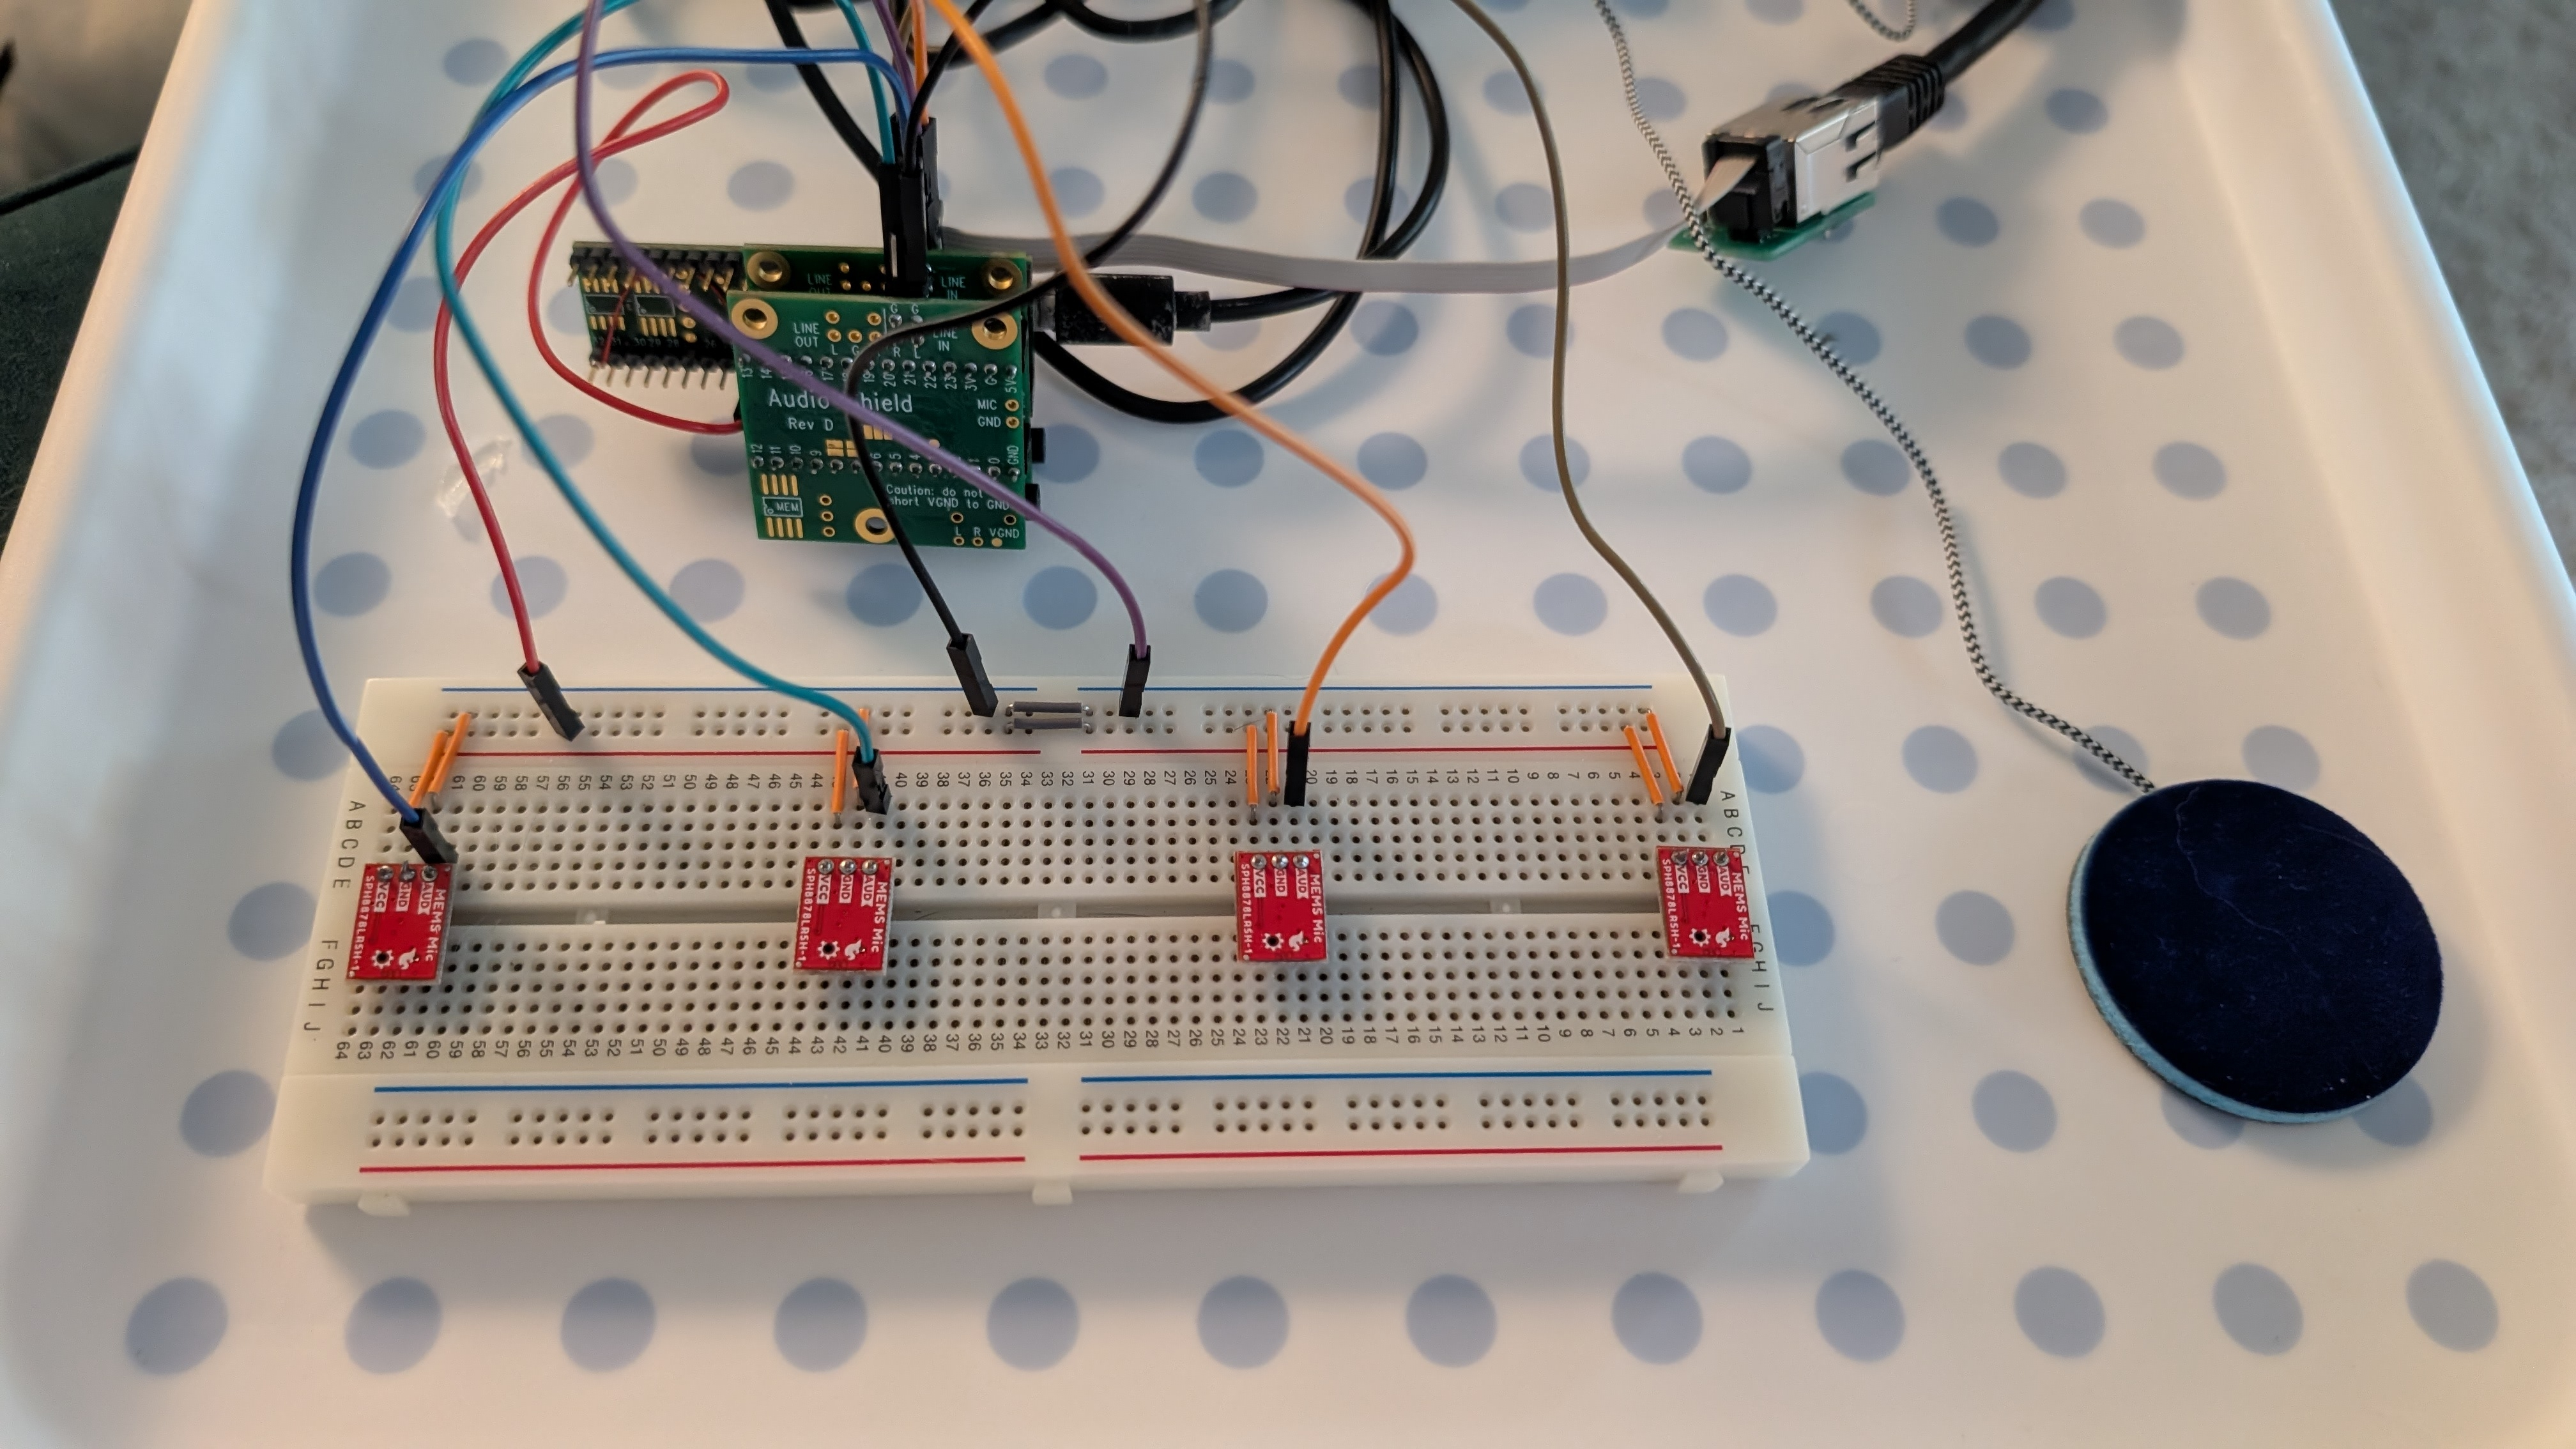
\includegraphics[width=0.95 \textwidth]{figures/hardware_01.jpeg}
		\caption{Left: Sparkfun analog MEMS microphones. Right: Speaker}
	\end{figure}
\end{frame}

\begin{frame}{Hardware Implementation - Phase Check}
	\begin{itemize}
		\item Connect all 4 analog microphone input wires to the same microphone condenser unit
		\item Good way to confirm that all 4 analog audio channels are phase locked
		\item This is not a "given" for many circuits. There are many places an audio board can introduce (non-deterministic) lag
	\end{itemize}
\end{frame}

\begin{frame}%{Phase Check}
	\begin{figure}
		\centering
		\includegraphics[width=0.95 \textwidth]{figures/recording_phase_check_02.png}
		\caption{Phase Check - all 4 analog inputs sampling the same mic}
	\end{figure}
\end{frame}

\begin{frame}%{Phase Check}
	\begin{figure}
		\centering
		\includegraphics[width=0.95 \textwidth]{figures/recording_phase_check_01.png}
		\caption{Phase Check - all 4 analog inputs sampling the same mic}
	\end{figure}
\end{frame}


\begin{frame}{Hardware Implementation - Linear Distance Measurement}
	\begin{itemize}
		\item Arrange all 4 mics in a straight line with known distances (50.4mm) between them
		\item We should be able to measure the distance between the mics using our algorithms*
	\end{itemize}
\end{frame}

\begin{frame}%{Linear Arrangement}
	\begin{figure}
		\centering
		\includegraphics[width=0.95 \textwidth]{figures/recording_linear_arrangement_03.png}
		\caption{Linear Arrangement - all mics in a line}
	\end{figure}
\end{frame}

\begin{frame}%{Linear Arrangement}
	\begin{figure}
		\centering
		\includegraphics[width=0.95 \textwidth]{figures/recording_linear_arrangement_02.png}
		\caption{Linear Arrangement - all mics in a line}
	\end{figure}
\end{frame}


\begin{frame}%{Linear Arrangement}
	\begin{figure}
		\centering
		\includegraphics[width=0.95 \textwidth]{figures/recording_linear_arrangement_01.png}
		\caption{Linear Arrangement - all mics in a line}
	\end{figure}
\end{frame}


%channels 0&1: mic[0].time_idx: 20985245-0.02[], mic[1].time_idx: 20985240-0.89[], TDOA: 133.07us, linear_intra_mic_distance: 45.64mm
%channels1&2: mic[1].time_idx: 20985240-0.89[], mic[2].time_idx: 20985233-0.78[], TDOA: 156.21us, linear_intra_mic_distance: 53.58mm
%channels 2&3: mic[2].time_idx: 20985233-0.78[], mic[3].time_idx: 20985225-0.13[], TDOA: 166.68us, linear_intra_mic_distance: 57.17mm
%channels 0&2: mic[0].time_idx: 20985245-0.02[], mic[2].time_idx: 20985233-0.78[], TDOA: 289.28us, linear_intra_mic_distance: 99.22mm
%channels 0&3: mic[0].time_idx: 20985245-0.02[], mic[3].time_idx: 20985225-0.13[], TDOA: 455.96us, linear_intra_mic_distance: 156.39mm
%channels 1&3: mic[1].time_idx: 20985240-0.89[], mic[3].time_idx: 20985225-0.13[], TDOA: 322.89us, linear_intra_mic_distance: 110.75mm
%
%
%chirp detected between channels 0&1: mic[0].time_idx: 3048808-0.57[], mic[1].time_idx: 3048814-0.06[], TDOA: -147.46us, linear_intra_mic_distance: -50.58mm
%chirp detected between channels 0&2: mic[0].time_idx: 3048808-0.57[], mic[2].time_idx: 3048821-0.63[], TDOA: -293.38us, linear_intra_mic_distance: -100.63mm
%chirp detected between channels 0&3: mic[0].time_idx: 3048808-0.57[], mic[3].time_idx: 3048827-0.51[], TDOA: -432.10us, linear_intra_mic_distance: -148.21mm
%chirp detected between channels 1&2: mic[1].time_idx: 3048814-0.06[], mic[2].time_idx: 3048821-0.63[], TDOA: -145.91us, linear_intra_mic_distance: -50.05mm
%chirp detected between channels 1&3: mic[1].time_idx: 3048814-0.06[], mic[3].time_idx: 3048827-0.51[], TDOA: -284.64us, linear_intra_mic_distance: -97.63mm
%chirp detected between channels 2&3: mic[2].time_idx: 3048821-0.63[], mic[3].time_idx: 3048827-0.51[], TDOA: -138.72us, linear_intra_mic_distance: -47.58mm
\begin{frame}[fragile]{Linear Distance Measurement}
	
	\begin{figure}
		\centering
		\[
		\begin{array}{c c|cccc}
			& & \multicolumn{4}{c}{\mathbf{B}} \\
			& & \multicolumn{4}{c}{\rule{0pt}{0.5em}} \\[-1em]
			& & ch0 & ch1 & ch2 & \cellcolor{red!20}ch3 \\ \hline
			& ch0 &       & 50.58  & 100.63 & \cellcolor{red!20}148.21 \\
			\mathbf{A} & ch1 &       &        & 50.05  & \cellcolor{red!20}97.63  \\
			& ch2 &       &        &         & \cellcolor{red!20}47.58
		\end{array}
		\]
		
		
		
		
		
		\caption{$\Delta t$ between channels A and B}
	\end{figure}
	
	\vspace{-0.5em}
	
	\begin{itemize}
		\item Runtime: $\approx 222\,\mu\mathrm{s}$ per channel
		\item Total runtime  $< 1\,\mathrm{ms}$ for all 4 channels
		\item 8-channel audio lets gooooo
	\end{itemize}
	
\end{frame}






